%%%%%%%%%%%%%
%  Ch1 : Generalities  %
%%%%%%%%%%%%%

\chapter{Fundamental principles of acoustics}
\section{Definition and origin of sound}
	\begin{wrapfigure}[9]{l}{5.5cm}
	\vspace{-6mm}
	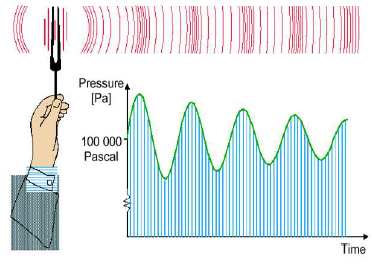
\includegraphics[scale=0.5]{acoustics/ch1/1}
	\captionof{figure}{}
	\label{fig:1.1}
	\end{wrapfigure}	
	Vibration when a mechanical excitation is applied on a material, air or water is the main source of sound. We speak about sound when the vibrations in air are perceptible by ear. The example on \autoref{fig:1.1} illustrates the vibration of a tuning fork that induces over- and under-pressure in the air around (order of magnitude small compared to ATM). Air particles are moving and describe a wave, a longitudinal wave, meaning that the particles displacement is parallel to the wave direction. Man can hear sound frequencies between 20Hz-20kHz, below we speak about infra-sound and above the limit, about ultra-sound.  
	
\setcounter{section}{4}
\section{Sound levels}
\subsection{The effective sound pressure}
	The sound perceived with a constant loudness may be both a pure sine tone and a stochastic sound generated by a source: p(t) is extremely complicated, and yet the human ear have the impression of a constant loudness. The ear seems to be sensitive to the energy of sound waves. This led to the consideration of the \textbf{effective–} or \textbf{Root-Mean-Square (RMS)} value of the sound pressure, over a certain time interval, as an measure of
intensity:

	\begin{equation}
	p_{eff} = \sqrt{\frac{1}{t_2 - t_1} \int _{t_1}^{t_2}p^2(t) \, dt}
	\end{equation}